% Turabian Formatting for Theses and Dissertations, 2018/08/06
%
% Developed using the turabian-formatting package (2018/08/01), available through CTAN: http://www.ctan.org/pkg/turabian-formatting
%
% Additional document class formatting options:
%
% raggedright: ragged right formatting without hyphenations
% authordate: support for the author-date citation style
% endnotes: support for endnotes

% document class handles the big-picture formatting
\documentclass{turabian-thesis}

% fancyhdr does fancy headers
\usepackage{fancyhdr}

% microtype handles microscopic improvements
\usepackage{microtype}

% graphicx handles graphics
\usepackage{graphicx}

% cmap makes pdfs searchable
\usepackage{cmap}

\usepackage[utf8]{inputenc}

% csquotes handles quotations
% ellipsis handles ellipses... obviously.
\usepackage{csquotes, ellipsis}

% allows half and half in tables.
\usepackage{diagbox}

% allows multiple rows
\usepackage{multirow}

% Specify paper size with geometry package
% \usepackage[pass, letterpaper]{geometry}

% For citations, use the biblatex-chicago package
\usepackage{biblatex-chicago}
\addbibresource{backmatter/works-cited.bib}

% For fancier tables.
\usepackage{booktabs}

% For left-aligned
% \usepackage[document]{ragged2e}

% For lorem ipsum text. use \lipsum[5] to create placeholder text.
% Very handy to get an overview of how it's going to look, but also can make you feel unreasonably confident- beware!
\usepackage{lipsum}


% Information for title page
\title{Harmonic Based Extended Techniques and their Compositional Applications}
\subtitle{An Investigation in New String Technique}
\author{Rhys Gray}
\date{\today}


% this is where the document starts. Comment out things that you don't need.
\begin{document}

\frontmatter{}
\maketitle
\cleardoublepage{}
\section[Declaration]{Declaration}
\vspace*{\stretch{1}} \noindent I declare that all material in this exegesis is my own work except where there is clear acknowledgement or reference to the work of others and I have read the University statement on Academic misconduct (Plagiarism) on the University website at
\url{www.utas.edu.au/plagiarism} or in the Student Information Handbook. I further declare that no part of this paper has been submitted for assessment in any other unit at this university or any other institution. I consent the authority of access to copying this exegesis. This authority is subject to any agreement entered into by the University concerning access to the exegesis. 
\vspace*{\stretch{2}}

Rhys Gray

\date{\today}

\thispagestyle{empty}
\cleardoublepage{}

\chapter*{Abstract}

I propose to explore a range of extended techniques that utilise the harmonic series and assess how they can be used in my, and other people’s, creative practice. These techniques include (but are not necessarily limited to) multiphonics, subharmonics, and audio-processed harmonics. Due to the scope of this project, stringed instruments will be the primary focus. For the purposes of brevity, these harmonic-based extended techniques will simply be referred to as 'techniques' throughout the paper, except for when differentiation between standard techniques is needed. 

While some techniques such as harmonics are well established and understood, others, such as subharmonics, are still immature in terms of both repertoire and resources available.  The timbral potentials of these techniques are uncharted territories and collectively represent a whole sound world that remains relatively inaccessible to contemporary art music composers.

To ensure that only new ground is covered, I will conduct a review of the literature and resources that are readily available to composers to assess what techniques require further investigation and refinement. By researching these techniques and the mechanics behind them, interviewing professionals, and analysing recordings made, I hope to gain a better understanding of how these techniques can be implemented in my practice. As part of both the analysis of techniques and my compositional practice, I will assess not only the compositional potential, but also the practicality of techniques. Reviewing the feasibility and notational aspects of the techniques will render the exegesis a practical document to reference when researching whether to include a technique.

I aim for my resulting exegesis to become a useful reference source for artists interested in learning about the mechanics, qualities, and potential implementations of these harmonic based extended techniques. The works that I compose accompanying the exegesis will show idiomatic treatment of the techniques and serve as references as such in the exegesis. The dissemination of the material I research will contribute to the accessibility of new sound possibilities for artists.
\cleardoublepage{}
\begin{center}
	\vspace*{\stretch{1}}
	
	Thank you to my supervisor, Matthew Boden, and my teachers Dr.\ Maria Grenfell and Dr.\ Scott McIntyre for their help and guidance. 
	I am indebted to my music teachers, Sally Ward and Glenn Schultz for inspiring my passion in music, and my peers and friends at UTas who have supported me in my research, and kept that passion alive. 
	My love and thanks go to my partner Claire Farrell\footnote{Whose cakes, biscuits, and mugs of coffee nourished me, and whose hugs and words of encouragement kept me sane. And vice versa.}
	, my family, and my cats Buttercup and Millie\footnote{Although they didn't do very much.}.
	
	\vspace*{\stretch{2}}
\end{center}
\cleardoublepage{}

\tableofcontents{}
\listofillustrations{}

\mainmatter{}
\section{Introduction}
\addcontentsline{toc}{chapter}{Introduction}


% Set page numbering to arabic the first time we commence a chapter.
% This is required to get the page numbering correct.
\pagenumbering{arabic}
\doublespace{}

I propose to explore a range of extended techniques that utilise the harmonic series and assess how they can be used in my, and other people's, creative practice. 
These techniques are multiphonics, subharmonics, and half-harmonics, confined to string based instruments due to the scope of this exegesis.
For the purposes of brevity, these harmonic-based extended techniques will simply be referred to as `techniques' throughout the paper, except for when differentiation between standard techniques is needed.

While some techniques such as harmonics are well established and understood, others, such as subharmonics, are still underdeveloped in terms of both repertoire and resources available. 
The timbral potentials of these techniques are uncharted territories and collectively represent an entire sound world that remains relatively inaccessible to composers.
% TODO: Evidence for uncharted territories - https://trello.com/c/u605dDsM/15-evidence-for-uncharted-territories

% To identify where further research is required, I will conduct a review of the literature and resources that are readily available to composers to assess what techniques require further investigation and refinement. 
% By researching these techniques and the mechanics behind them, interviewing professionals, and analysing recordings made, I hope to gain a better understanding of how these techniques can be implemented in my practice. 
% As part of both the analysis of techniques and my compositional practice, I will assess not only the compositional potential, but also the practicality of techniques. 
% Reviewing the feasibility and notational aspects of the techniques will render the exegesis a practical document to reference for performance and composition.

I aim for my resulting exegesis to become a useful reference source for artists interested in learning about the mechanics, qualities, and potential implementations of these harmonic based extended techniques. 
The works that I compose accompanying the exegesis will show idiomatic treatment of the techniques and serve as references as such in the exegesis.
This exegesis makes use of hyperlinks throughout to promote its use as a reference document. 
The dissemination of the material I research will contribute to the accessibility of new sound possibilities for artists.
% chapter1.tex (Chapter 1 of the thesis)


% define new commands i.e. variables i.e. pieces of music
\newcommand{\violinPiece}{\emph{what are you doing with the humans}}
\newcommand{\violaPiece}{\emph{doppelganger}}
\newcommand{\bassPiece}{\emph{the veldt}}
\newcommand{\celloPiece}{\emph{liminal}}
% aliases for performers to maintain anonymity
\newcommand{\violaParticipant}{Angus}
\newcommand{\celloParticipant}{Sarah}
\newcommand{\bassParticipant}{Joe}
\chapter{Literature Review and Methodology}

\section{Literature Review}
This study builds on and contributes to the catalogue of resources available to composers interested in implementing harmonic based extended techniques in their practice. 
The topic of `harmonic based extended techniques and their compositional applications' is broad, and I will be unable to explore the entire corpus of techniques available to all instruments as this falls outside the scope of this exegesis. 
This is by design, as certain instruments lack certain facets of research, while others are already well documented, the most obvious example being string harmonics, which are common practice. 
This broad topic affords a certain level of flexibility to explore what is both novel and feasible given my available resources, all under the unifying theme of harmonic based extended techniques.

Many of the techniques that this study deals with are still in their comparative infancy, especially notationally.
% TODO: Evidence for techniques notational infancy -
% https://trello.com/c/vxCdj0rV/16-evidence-for-techniques-notational-infancy
%??? Not really sure why it is *subjective*.
As such, engraving the works produced in the course of this study is a more subjective matter, rather than the well-established practice that it normally is due to the lack of a myriad of scores to draw reference from. 
A review of the available literature makes it clear that attempts have been made to standardise contemporary music notation, but have either fallen short, or are now outdated. 
Kurt Stone organised an international conference on new musical notation in 1974 in Ghent, Belgium, and then produced the treatise \emph{Music Notation in the Twentieth Century} in 1980 as a result of the conference.\autocite[xiii]{stoneMusicNotationTwentieth1980} 
This, along with Gardner Read’s 1979 \emph{Music Notation}, served as a strong base for the standardisation of music notation, but both are mired by their age and computer-based notation not being widespread.\autocite{readCompendiumModernInstrumental1993} 
% TODO: Formatting of Gardner needs to comform to Turabian - https://trello.com/c/nGe6QdQm/18-formatting-of-gardner-needs-to-comform-to-turabian
%??? ... many ... Is it really *many*?
It is therefore unsurprising that both omit the notation of stringed multiphonics, subharmonics, and half-harmonics, the bulk of the research largely postdating publication. 
Elaine Gould’s 2016 book \emph{Behind Bars} immediately became the gold standard of engraving manuals, her decades of notational and editorial experience at Faber Music lending weight to her comprehensive treatise.\autocite[]{gouldBars2011} 
But the same new techniques are omitted from Behind Bars, with Gould stating: 
\begin{quotation}
 ‘I have been highly selective in the choice of extended instrumental and vocal techniques included in this book, but it is intended that this should give the reader the facility to create notation for other techniques not in common use.’\autocite[iii]{gouldBars2011} 
\end{quotation}
% TODO: Double check formatting for indented paras re Turabian - https://trello.com/c/hvstPkHd/17-double-check-formatting-for-indented-paras-re-turabian
Gould’s book is less proscriptive than its forerunners, and focuses more on creating a consistent style language, providing the reader with the tools of standardised and codified ‘common practice’ notation to build new extended technique notation. 
As such, for all notational aspects, I will be drawing upon the Gould for the philosophy of engraving, if not exact notation, which has the benefit of almost forty years of usage and review against its peers.

Gould provides the tools which Ellen Fallowfield uses to construct a notation method for string multiphonics in her PhD ‘Cello Map’, the framework of which this exegesis will follow. 
A detailed, process-oriented review of technique informs the creation of resources which are then analysed.\autocite{fallowfieldCelloMapHandbook2009} 
Fallowfield’s analysis produced the website cellomap.com, a manual of techniques for performers to use. 
She states that her text maps:
\begin{quotation}
% TODO: format quote properly - https://trello.com/c/ajbnCQMe/19-format-quote-properly
    [\ldots] “actions that a cellist can make” onto “sounds that a cello can produce”. 
    In other words, we have tried to reduce the cello and cellist to scales of actions and sounds, and show how cellists can influence sound (loudness, overtone content, pitch…) by their actions (bow speed, contact point, stopping position…). 
    This standpoint is a deliberate move away from providing performers and composers with catalogues of special effects and extended techniques. 
    Instead, we would like to provide information about how the cello works that can serve the imagination of performers and composers.\autocite{fallowfieldCelloMap}
\end{quotation}
This approach ‘future proofs’ her thesis by abstracting the elements into their most base form, showing all of the sounds a cello can make using all of the actions a cellist can perform. 
While the website is comprehensive, Fallowfield seemingly avoids making any judgement calls on the compositional applications of the techniques that she reviews, and the reader is left to draw their own conclusions on the compositional effectiveness of any given technique. 
Fallowfield does, however, note that a repertoire gap exists for etudes exploring multiphonics for the cello, and indeed, the entirety of the string family. 
As part of my practice-led research, it seems fitting to compose a piece that begins to address this repertoire gap.
% TODO: Footnote for reference for the 'entirety of string family' - https://trello.com/c/KAmvtp1D/20-footnote-for-reference-for-the-entirety-of-string-family

% Bertram Turetzky’s book, \emph{The Contemporary Contrabass} was written to exemplify the contrabass as a serious solo and melodic instrument, which was underrepresented in the literature.\autocite[]{turetzkyContemporaryContrabass1974} He theorised: 

Bertram Turetzky’s book, \emph{The Contemporary Contrabass} was written to exemplify the contrabass as a serious solo and melodic instrument in response to the double bass's underrepresentation in the literature.\autocite[]{turetzkyContemporaryContrabass1974}

He theorised: 
\begin{quote}
 ‘[…] Concertizing Was The Key, which in the 1950’s was impossible mainly due to the lack of literature. I attacked this problem in two directions: 1. Locating original contrabass music from the eighteenth and nineteenth centuries, and 2. Commissioning twentieth century music.’\autocite[vii]{turetzkyContemporaryContrabass1974}
\end{quote}
His practice-led research centered on seeking to understand the techniques that contemporary composers could use in solo contrabass repertoire. 
Turetzky deliberately omitted including any guidance or judgements on notation, or categorisations of the difficulty of the techniques, stating that \begin{quote}
 ‘[…] the time between this printing and the second edition will suffice to suggest and select the best notational concepts from a more substantial literature than we possess now.’\autocite[ix]{turetzkyContemporaryContrabass1974} 
\end{quote} The second edition saw Turetzky call for more experimentation with multiphonics, stating:
\begin{quote}
 ‘I know of no music employing string multiphonics […] this is entirely new ground, it remains for composers and performers to build the usable technique.’\autocite[138]{turetzkyContemporaryContrabass1992}
\end{quote}
The specification of both composers and performers being needed to ‘build the usable technique’ is peculiar, until one re-examines the context in which Turetzky knew of these techniques. 
Thus, we might infer that he was attempting to address the situation through commissioning new literature.

Performers and researchers such as Fallowfield are necessary to establish the technique, but it is impossible for a ‘usable technique’ to be built without composers implementing their research and contributing to a pool of repertoire to show the correct usage of the technique.
% TODO: Howell book has many omissions- explain those omissions - https://trello.com/c/7R9ZKD4X/21-howell-book-has-many-omissions-explain-those-omissions

% Thomas Howell’s 1974 book, \textit{The Avant-Garde Flute} followed Turetzky’s contrabass technique book, as part of Turetzky’s \emph{The New Instrumentation} series, which was published by California Press until Scarecrow Press took over in 2004.\autocite[4]{fallowfieldCelloMapHandbook2009} 
% It is relatively conservative in its content, and has many omissions. 

Robert Dick’s \emph{The Other Flute} was released in 1989, and was notably used as the primary reference for microtonal flute fingerings by John Cage in the preface to his piece \emph{Music For}.\autocite{cageMusicPartsVoice1984} 
\emph{The Other Flute} is a thorough performance technique manual, presenting each fingering and its resultant multiphonics one after the other, using a chart of descriptions to specify the qualities.\autocite[86--135]{dickOtherFlute1989} 
It specifies the following: ‘exact pitch, ease of response, starting time, stability, dynamic range, timbre, and, if present, noise level, residual tone, and degree of modulation.’\autocite[84]{dickOtherFlute1989} 
While this text focuses more on instruction, it is an efficient system, and sorts the multiphonics into four classes graded by difficulty. 
% The multiphonics are presented in order of their method of production; multiphonics derived from natural harmonics, from fingerings of chromatic pitches, and those based on microtonal segments. 
% The scope of my research is limited to the multiphonics based on natural harmonics. 
From the perspective of a composer, Dick’s book provides ample resources on the qualities of each multiphonic, but generic descriptions of their characteristics: enough for a composer to assess whether any given multiphonic is worth investigating with a flautist. %%??? Semicolon changed to colon. 
While the scope of my research focuses on stringed instruments, Dick’s method of cataloguing the qualities is a logical and comprehensive model to follow.
% TODO: Reference for The New Instrumentation series - https://trello.com/c/CQOIRJBQ/22-reference-for-the-new-instrumentation-series

\emph{The Contemporary Violin} is one of the more recent books in Turetzky’s \emph{The New Instrumentation} series.\autocite[]{strangeContemporaryViolinExtended2001} 
It provides a comprehensive review of various violin techniques, but attempts to shy away from any implication of notational authority, most notably in the section on multiphonics, which seems to contradict rules codified by Gould (though to be fair, the Gould postdates Strange).\autocites[134]{strangeContemporaryViolinExtended2001}[257--258]{gouldBars2011} 
Fallowfield identified issues with the presentation format of \emph{The Contemporary Violin} in the literature review of her thesis: 
\begin{quotation}
 ‘The reader will find [information about \textit{col legno battuto}] under the first chapter heading: ‘Bowing Technique’, the subheading ‘Col legno battuto’. Later, chapter three: ‘Percussion Techniques’ includes the subheading ‘The Bow’, in which \textit{col legno battuto} is described again.’\autocite[12]{fallowfieldCelloMapHandbook2009}
\end{quotation}
Though the scope of my study is significantly smaller in scale, presentation of the findings is paramount to maintain accessibility as a resource. 
Given that my study focuses on harmonic based extended techniques, an overlap with techniques such as multiphonics is possible, and therefore needs to avoid the structural pitfalls of Strange’s layout where information is repeated. 
Fallowfield’s later concern of a need for a balance between subjectivity and level of detail when describing technique and sound is also relevant to both the Strange book and doubly so to the study. 
These manuals merely describe the qualities of various techniques, whereas my study will be dealing with the compositional applications of the techniques. 
Taking the extra-musical content such as blending, appropriateness for use in pitch sets, and other aspects of composition into account poses a threat to the usability of my study due to information overload. 
Marcus Weiss and Giorgio Netti discuss the reasons for limiting their study to extended techniques in the introduction to their book \emph{The Techniques of Saxophone Playing}, stating ``It might indeed be conceivable to compile a multi-dimensional “Encyclopaedia of Saxophone Playing” [, however] the demands on presentation and readability would be so complex as to make such a text impractical``.\autocite[Introduction]{weissTechniquesSaxophonePlaying2010}

So far, all of the literature reviewed (with the exception of the Gould and other engraving manuals) has been written either with the performer in mind, or has been written by an instrumentalist. 
Much of the composer-focused literature is found in the form of orchestration manuals, such as Samuel Adler’s \emph{The Study of Orchestration} and Walter Piston’s \emph{Orchestration}.\autocite{adlerStudyOrchestration2002, pistonOrchestration1969} 
Attempting to cover the breadth of the art of orchestration, let alone composition, necessitates the omission of extended techniques. 
This is the inverse of the issue Weiss and Netti encountered, where their study required an omission of ground-level theory regarding the technical aspects of saxophone playing. 
Read’s \emph{Compendium of Modern Instrumental Techniques} touches upon multiphonics, but delegates to Dick, Thomas Howell, and many of the other books from Turetzky’s \emph{The New Instrumentation} series for notation and structure.\autocite[160]{readCompendiumModernInstrumental1993} 
It becomes apparent that no matter the author, instrument, or technique, the work of packaging extended technique information for composers is left to somebody else. 
Composers seek to cover the entirety of the craft, while performers seek to cover the entirety of the instrument. 
Therefore, there is a dearth of resources for composers seeking to incorporate harmonic based extended techniques into their practice. 
My study addresses this by covering the playability, notation, and implementation of these techniques. 
Through practice-based research, the exegesis produced by my study will document the process of composing using these techniques, refining the methodology and notation through the creation of several new works. 
The resulting document will fill a hole in literature aimed at composers by acting as a practical manual for those interested in implementing harmonic based extended techniques in their own practice.


\newpage

\section{Methodology}
My research topic “Harmonic Based Extended Techniques and their Compositional Applications” is a review of techniques, and how they can be incorporated in my own practice. 
As such, it is highly subjective, and the research methodology --- largely qualitative --- reflects this. 
Quantitative research, such as the analysis of documents using the same techniques will be used to support subjective claims. 
Each technique will be reviewed individually, as they are discrete from one another. 
Because many of the techniques are uncommon or difficult, consultation with players is paramount to undertake a fair assessment of the techniques. 
Document analysis of technique manuals will augment oral history research into the qualities and attributes of techniques.

To make an educated opinion on the value of a technique, data must first be collected. 
Compilation of techniques both in isolated, controlled environments, and in context in musical works will allow a full and accurate use of the analytical method on recordings. 
% Using a Fast Fourier Transformation as in Riera’s thesis on saxophone multiphonics, the prominent harmonics of each technique will be uncovered, for harmonic analysis.\autocite{rieraComparativeStudySaxophone2014} 
Examination of techniques in musical context will allow for value judgements to be made about the musical effectiveness of the technique. 
The recorded data will be treated, and then interpreted and analysed, with the results being implemented in new works.\autocite{torresMultiphonicsCompositionalElement2012} 
Through this process, my research will feed into my practice.


A holistic approach, taking both the sound possibilities and the player implications (“is this technique too difficult for the average player?”, “do I need to write for specific artists if I want to use this technique?”, etc.) is necessary to evaluate its overall potential for incorporation in my practice. 
To overcome this, oral history methodology will be used to gather first-hand experiences and opinions on techniques. 
In Barnett’s ``Aspects of Vocal Multiphonics'', she conducts several interviews with singers to better understand the way the technique functions from a performer’s perspective.\autocite{barnettAspectsVocalMultiphonics1977} 
% TODO: Check thesis citation format - https://trello.com/c/yFoIKvKg/23-check-thesis-citation-format
Interviewing musicians able to play these techniques will deepen my understanding of the mechanics and technical aspects of implementing these techniques. 
% While my research is concerned with how I personally can incorporate these techniques into my practice, an effort to interview peer composers will be made, especially those that share common compositional traits with me. 
% Their experiences with composing for these extended techniques will provide more data points to draw comparisons from, and contemporary composer’s compositions and feedback were a valuable component of Dr.\ Sarah Watts’ thesis to assess the effectiveness of the techniques.

Augmenting the interviews, document analysis will be used on technique manuals that detail the production and quality of techniques. 
By building off the framework of classification articulated in Robert Dick’s seminal \emph{The Other Flute} and adapting it to accommodate a variety of techniques, comparisons across different techniques will be able to be made.\autocite{dickOtherFlute1989} 
Through this, an understanding of the technical and mechanical aspects of the techniques will be gained. 
Techniques will be assessed on their practicality, ease of use, timbral qualities, and compatibility with my practice. 
Notation for the techniques varies from composer to composer, and where a common notational standard has not been developed (such as subharmonics), a document analysis of current notational standards will be undertaken, making reference to Gould’s seminal text on music notation, \emph{Behind Bars}.\autocite{gouldBars2011} 
Through this, and subsequent consultation with players, development of a consistent and effective notational language can be achieved.

This process of practice-based research will feed into itself, forming a research-based practice as detailed in Hazel Smith and R.\ T.\ Dean's ``Practice-led research, research-led practice in the creative arts'', where the value of it is described as: \begin{quotation}
    the possibility [that] new knowledge \ldots may be generated by moving from a stance more accurately seen to move from the `unknown to the known' whereby imaginative leaps are made into what we don't know as this can lead to critical insights that can change what we do know.\autocite[48]{smithPracticeledResearchResearchled2009}
\end{quotation}
This iterative process will help clearly define the scope of the exegesis, and provide further insight into existing technique, as well as help `build the new techniques'.

Through the collection of data from a multitude of sources and a range of different methods, it will become evident how harmonic based extended techniques are to be treated idiomatically. 
By undertaking a holistic review of the techniques including the player's point of view, the qualitative research I perform will enable not only me to incorporate these techniques into my own practice, but future composers that are interested in these techniques.

% \newpage
% \section{New Section}
% Here we have started a new page to show how the headers work. The
% text in the header should be the last section title declared at
% the end of the current page.

% This new paragraph shows how to set\index{index items}index items
% and\index{index items!subindex items} subindex items.

% \subsection{New Subsection}
% Here's a subsection with some simple maths $a^2+b^2=c^2$.

% \subsubsection{subsubsection}
% Here's a\index{subsubsection}subsubsection\ldots oooooooohh wow
% wee!!!!!!

% \newpage
% Some more text to check indent and show how references work



% And finally, here's a table example (Table \ref{tab:taba}).
% \begin{table}[hbtp]
% \begin{center}
% \begin{tabular}{|r|r|r|r|r|}
% \hline
% $n=$&2&3&4&5\\
% \hline
% $c$ (rad/day)&1.67&0.52&0.06&-0.17\\
% \hline
% period (days)&3.75&12.00&100.00&37.50\\
% \hline
% \end{tabular}
% \end{center}
% \caption{\label{tab:taba}A simple table}
% \end{table}

% chapter2.tex (Chapter 2 of the thesis)

\chapter{Assessment of Harmonic Based Techniques and Repertoire}

% //TODO: Talk about Pythagoras - https://trello.com/c/uo0AALKP/1-talk-about-pythagoras
Goals for this chapter:

1. Explain sound production of stringed instruments.
2. Explain the way in which the techniques differ from standard sound production.
3. Explain the qualities of the techniques.
4. Explain the notation.



Harmonic based techniques invariably make use of the harmonic series in one way or another. 
The harmonic series is a sequence of tones in which the frequency of each is an integer multiple of the fundamental frequency. 
The earliest forms of tuning systems were based around these, but modern instruments are tuned using equal temperament. 
The pitch of sound on stringed instruments is determined via tension, effecting the speed (and consequently pitch) the string vibrates at. 
Altering the tension is most commonly achieved via fingerings on the instrument's fingerboard, but bow pressure can also play a part in pitch production (see subharmonics).

The objective categorisation of techniques is a Sisyphean task due to the variability of the techniques, but general guidelines can be made; Dick's \emph{The Other Flute} makes good use of quantifying qualitative data about the properties of multiphonics, and the idea of his tables will be used, adapting the format to each technique.\autocite[84]{dickOtherFlute1989}

To be able to pass any judgement on the techniques, we must first understand these techniques' capabilities, limitations, qualities, considerations, and values. 
Without references to other composers' works, any implication of authority on what constitutes as `idiomatic' writing is baseless. 
As such, references to other works will be used to support claims. 
Where no such references are available, it will be marked as the author's personal opinion. 
Even without any available references to substantiate compositions as idiomatic, their creation contributes to the literature, and thus can be used if not as an example, a warning on what not to do. 

\subsection{Background}
All of the techniques covered in this exegesis involve the excitation of a string instrument's string in a non-standard way. 
A small amount of understanding the physics behind these techniques is required, though they are not fully understood.
Strings create sound via the Helmholtz motion, which 

Subharmonics are perhaps a misnomer, and do not \emph{technically} fall under the branch of harmonic based techniques.
This is because their production is not by ways of the overtone (or undertone) series, as the pitches that can be produced do not follow any discernable ratio based pattern.



% Provide an overlay of the techniques and explain how they work, the general benefits and such.
% \subsection{Research statement/problem}
% Techniques are under-developed and/or under-used.

% \subsection{Aim and scope of thesis}
% Examples of use in current literature will support use-case scenarios, dearths of usage will support the fact that they are underused.

% \subsection{Significance of work}
% The production of technique and its uses.
\newpage
\section{Subharmonics} \label{sec:subharmonicsDiscussion}
% TODO: Explain subharmonics - https://trello.com/c/HP0b1P3h/2-explain-subharmonics
First discovered by Mari Kimura, subharmonics are a type of overpressure which produces a sound lower than the fundamental.\autocite{kimuraHowProduceSubharmonics1999} 
When the bow is drawn across the string, the drag of the bow twists the string, creating torsional oscillation. 
Under the right conditions, these can interact with the string to produce an identifiable pitch lower than the fundamental.\autocite{Subharmonics2006} 
One of the newest string techniques, subharmonics are still in their comparative infancy, and their notation has not been formalised. 

Subharmonics represent an incredible opportunity for solo string repertoire. 
On higher pitched instruments, their use can provide harmonic support (particularly in cadenza passages) and extend the range of the instrument. 
On lower pitched instruments, subharmonics function better as a timbral mechanic, much like overpressure. 

Subharmonics are explored in my works \nameref{sec:bassPiece}, and \nameref{sec:violaPiece}.


\subsection{Subharmonics in the literature}

Subharmonics share a common relative with woodwind and brass instrument in pedal tones.
They operate in similar ways, though the method of production differs greatly, and the reliability of production of subharmonics is much lower than the equivalent on brass instruments.
Because of these commonalities, it is not unreasonable to make comparisons between subharmonics and its equivalents, especially in regards to notation and implementation in works.

Possibly the first person to make use of the technique, Crumb described what we know as subharmonics as `pedal tones'.\autocite{crumbBlackAngelsImages1971} 
The use of square noteheads and a separate stave for the resultant pitch makes the technique clear and readily understandable.\autocite[]{crumbBlackAngels1995}
\begin{figure}
    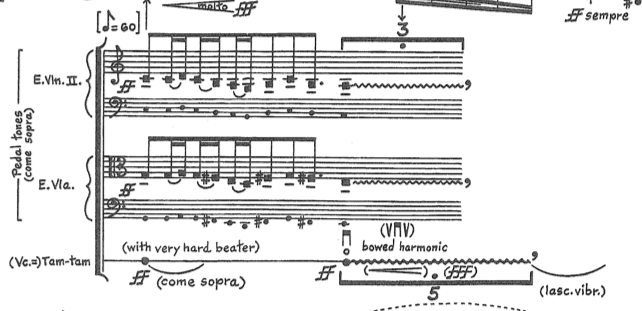
\includegraphics[width=\linewidth]{./resources/crumbBlackAngels.png}
    \caption{Excerpt from Crumb's \emph{Black Angels}}
    \label{fig:Excerpt from Crumb's Black Angels}
\end{figure}
% TODO: Citation is needed for Crumb - https://trello.com/c/Rpypkzbm/4-citation-needed-for-crumb
% TODO: Citation needed for pedal tones - https://trello.com/c/03arTJkS/5-citation-needed-for-pedal-tones



Gerard Grisey's \emph{Vortex Temporum} features overpressure, with a subharmonic of specifically a seventh.\autocite[]{griseyVortexTemporum}
He notates the subharmonic technique using a triangular filled notehead showing the intended pitch, along with a double down-bow, with an arrow above it, shown in \autoref{fig:Excerpt from Grisey's playing instructions for Vortex Temporum}. 
Somewhat abstracted out, this hides the intended effect behind symbols, and is slower to sight read.


\begin{figure}
  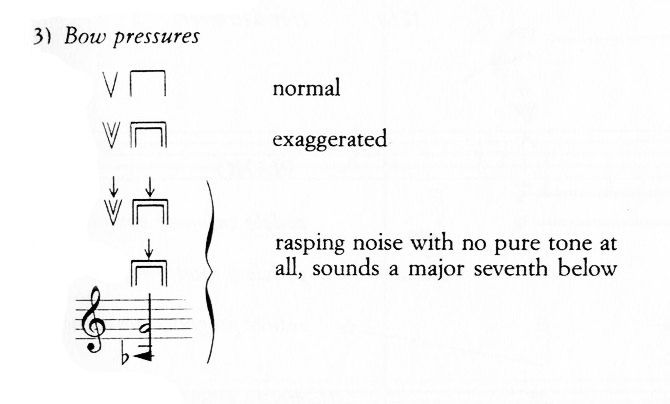
\includegraphics[width=\linewidth]{./resources/griseyVortexTemporum.jpg}
  \caption{Excerpt from Grisey's playing instructions for \emph{Vortex Temporum}.}
\label{fig:Excerpt from Grisey's playing instructions for Vortex Temporum}
\end{figure}


Mari Kimura's \emph{Gemini} (\autoref{fig:Excerpt from Kimura's Gemini}) is an example of idiomatic usage of subharmonics on the violin.\autocite[]{kimuraGemini1992}
Kimura's notation practice of using a harmonic denoting the intended pitch below the fundamental is similar to the standard notation of harmonics, which Gould states is to `write harmonics as the player will finger them.'\autocite[413]{gouldBars2011} 
Unfortunately, this method proved somewhat counterintuitive in practice, as the notation was too similar, and caused sight reading issues.

  
\begin{figure}
  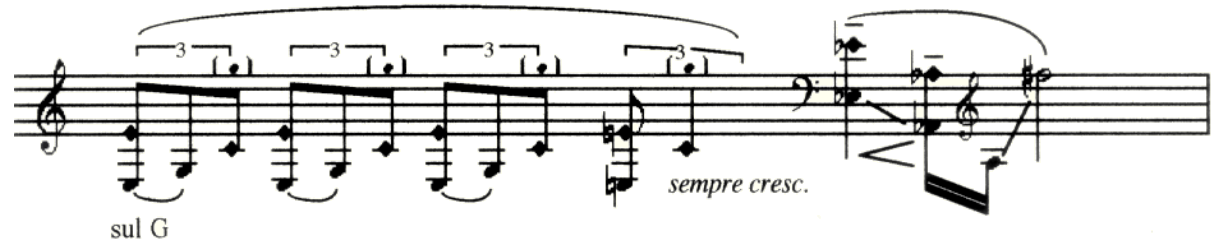
\includegraphics[width=\linewidth]{./resources/kimura_gemini.png}
  \caption{Excerpt from Kimura's \emph{Gemini}}\label{fig:Excerpt from Kimura's Gemini}
\end{figure}
% TODO: Citation needed for Gemini

  Botting notes that experimentations with octavic subharmonics yielded a pitch slightly flatter than an octave. He states \begin{quotation}
    `I developed a left hand finger technique whereby I rotate my hand slightly clockwise, pivoting on the finger stopping the string, which has the effect of sharpening the subharmonic enough to be more in tune with the fundamental.'\autocite[111]{bottingDevelopingPersonalVocabulary2019}
\end{quotation}

Players may find that subharmonics are easier on older strings, and they may also find that adding twists to the string may also help, or hinder the production of subharmonics, as shown in \autoref{tab:twistTable}.\autocite[]{kimuraHowProduceSubharmonics1999}

\begin{table}
  \centering
  \caption{Relation between twists in string and resultant subharmonics}
\label{tab:twistTable}
  \begin{tabular}{llllllll} 
  \toprule
  \multicolumn{1}{r}{} & \multicolumn{1}{c}{1/2} & \multicolumn{1}{c}{1} & \multicolumn{1}{c}{2} & \multicolumn{1}{c}{3} & \multicolumn{1}{c}{4} & \multicolumn{1}{c}{5} & \multicolumn{1}{c}{6}  \\ 
  \hline
  minor 2nd            & x                       & x                     &                       &                       &                       &                       &                        \\
  major 2nd            & x                       & x                     &                       &                       &                       &                       &                        \\
  minor 3rd            & x                       & x                     & x                     &                       &                       &                       &                        \\
  major 3rd            & x                       & x                     & x                     & x                     &                       &                       &                        \\
  perfect 4th          &                         &                       &                       & x                     & x                     &                       &                        \\
  diminished 5th       &                         &                       &                       &                       & x                     & x                     &                        \\
  perfect 5th          & x                       &                       &                       &                       &                       & x                     & x                      \\
  minor 6th            &                         &                       &                       &                       &                       &                       & x                      \\
  octave               & x                       & x                     & x                     & x                     & x                     &                       &                        \\
  \bottomrule
  \end{tabular}
  \end{table}

Sekulic describes subharmonics as:

\begin{quotation}
  `[\ldots] a sound that sounds an octave lower than g string. To produce this sound it is of great importance the use of bow [sic]- the place, speed, and pressure. It is however extremely unsustainable and unpredictable, thus it is difficult to use it much in the compositions.'\autocite[15]{sekulicYouHearMe2012}
\end{quotation}

Sekulic erroneously claims that subharmonics are solely producible on the G string, and can only produce an octave. 
Kimura's work, and my own experiments on a contrabass show that subharmonics are possible on any string, and octaves, major sevenths, and minor seconds are all readily achievable without specialist practice.\autocite[]{kimuraHowProduceSubharmonics1999}



\subsection{Notation of Subharmonics in the literature}

The example used on Long's website, \emph{The Modern Double Bass} (\autoref{fig:Notation of subharmonics from Long's website, The Modern Double Bass}) features a square notehead with the intended sound at pitch in a bracketed notehead, with harmonics and a technique line of `S.H'.\autocite[]{longSubharmonics2019}

\begin{figure}
  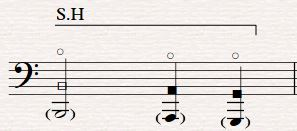
\includegraphics[width=\linewidth]{./resources/longSubharmonicNotation.jpg}
  \caption{Notation of subharmonics from Long's website, The Modern Double Bass}\autocite[]{longSubharmonics2019}
\label{fig:Notation of subharmonics from Long's website, The Modern Double Bass}
\end{figure}

It is the author's opinion that this is somewhat redundant, as just square noteheads with the intended produced pitch would be enough to delineate the technique. 
The technique line is supernumerary, and it would only be advisable to use it in extended passages of uninterrupted subharmonics.

% TODO: reference risset and rowe - https://trello.com/c/wDhTSCzs/29-reference-risset-and-rowe

Jean-Claude Risset's \emph{Variants}, written for Kimura, is a work that makes use of both subharmonics and digital processing of live sound.\autocite[]{rissetVariants1995}
It uses a separate stave for the subharmonics and digital processing, as seen in \autoref{fig:Excerpt from Risset's Variants}. 

\begin{figure}
  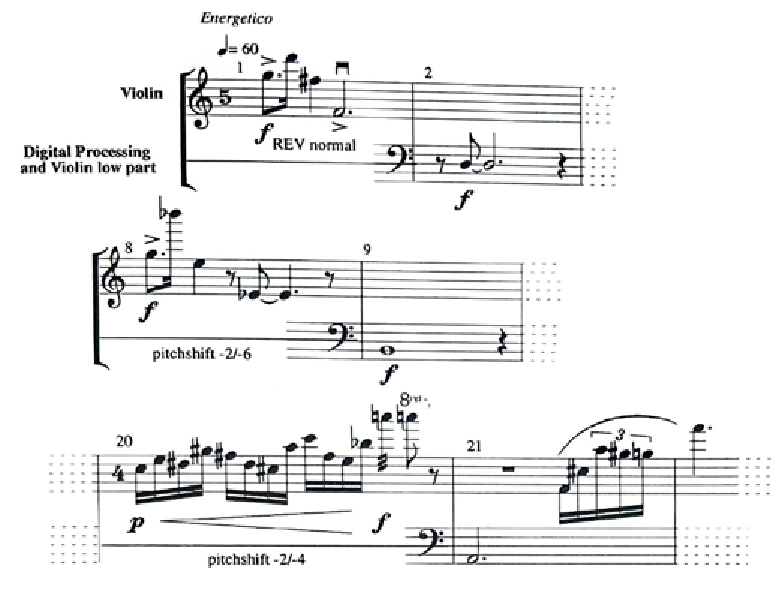
\includegraphics[width=\linewidth]{./resources/rissetALFExcerpt.pdf}
  \caption{Excerpt from Risset's \emph{Variants}}
\label{fig:Excerpt from Risset's Variants}
\end{figure}

Rowe also wrote a work for Kimura, and uses a regular notehead for fingering, with a square bracketed cue sized notehead, as seen in \autoref{fig:Excerpt from Rowe's Submarine}.\autocite[]{roweSubmarine1996}
This combines the best of both worlds, keeping the score free from clutter when not needed.
It should be noted that Rowe uses notation that has fallen out of style to notate \emph{normale} harmonics, notating the fingering position with the diamond notehead, and the resultant pitch with a harmonic circle above it. 
Harmonic circles always denote resultant pitch, and the inclusion of the fingering obfuscates this.\autocite[420]{gouldBars2011}


\begin{figure}
  \includegraphics[width=\linewidth]{./resources/roweALFExcerpt.pdf}
  \caption{Excerpt from Rowe's \emph{Submarine}}
\label{fig:Excerpt from Rowe's Submarine}
\end{figure}


% Musicians are better at sight reading above the stave than below the stave, so unlike natural harmonics, the need to split into another stave to show the resultant pitch is likely to be more common for composers wishing to use subharmonics. 



% TODO: undefined - https://trello.com/c/SU5ZEEmJ/6-- Do I need a citation for "musicians are better at sight reading above the stave than below"?
\newpage
\section{Multiphonics} \label{sec:multiphonicsDiscussion}
% TODO: Explain multiphonics - https://trello.com/c/6vkcY6CO/7-explain-multiphonics

Multiphonics are most commonly the domain of wind, and occasionally brass instruments, but they are an emerging technique in string writing. 
They are produced when fingerings split the string between two natural harmonics, allowing for the string to resonate at multiple frequencies.
% TODO: Citation needed for explanation of physics of multiphonics - https://trello.com/c/EboMHDaN/8-citation-needed-for-explanation-of-physics-of-multiphonics
Multiphonics on stringed instruments are difficult, but with appropriate preparation and notation, are feasible. 
Production of multiphonics, as with wind instruments, is not guaranteed, and can be dependant on a variety of external factors, including the humidity, make of the instrument, bow used, and other variables that are outside of the control of a composer. 
% TODO: Citation needed for the factors leading to multiphonics - https://trello.com/c/9iC7EAXb/24-citation-needed-for-the-factors-leading-to-multiphonics

Multiphonics are fragile, and require much preparation to execute reliably. 
Despite this, they can be used to achieve harmonies that are not otherwise achieveable through double-stopping, and lend themselves well to drawn out or slow passages of music. 
Multiphonics' exact pitching makes them ideal for music that uses ratios, microtones, or tone rows. 

Multiphonics are explored in my piece for violoncello, \nameref{sec:celloPiece}, and contrabass work \nameref{sec:bassPiece}.

\subsection{Multiphonics in the literature}

Fallowfield explores multiphonic production on the cello in her thesis CelloMap comprehensively, with video recordings of all possible multiphonics and permutations, including pizzicati.\autocite{fallowfieldCelloMapHandbook2009} 
These are isolated, though, and give little indication to the difficulty of the multiphonics.

Ashley John Long's `The Modern Double Bass' website serves a similar purpose as Fallowfield's CelloMap for the double bass.\autocite{longModernDoubleBass} 
He divides them into different categories as detailed in \autoref{tab:longTable}, some of which have more information and detail than others. 

\begin{table}[]
  \label{tab:longTable}
  \centering
  \resizebox{\textwidth}{!}{%
  \begin{tabular}{@{}ll@{}}
  \toprule
  \textbf{Type}                                      & \textbf{Description}                                                       \\ \midrule
  `Natural' multiphonics                             & Chart of different fingerings, similar to Fallowfield.                     \\ \midrule
  Pizzicato multiphonics                             & Description of technique, production, and result.                          \\ \midrule
  Textural multiphonics                              & Description of technique, production, result, and considerations.          \\ \midrule
  Multiphonics behind the bridge                     & Description of technique.                                                  \\ \midrule
  Artificial multiphonics                            & Chart of different fingerings, similar to Fallowfield.                     \\ \midrule
  Percussive multiphonics                            & Description of technique, production, result, and considerations.          \\ \midrule
  Timbral multiphonics                               & Description of technique.                                                  \\ \midrule
  Transformative multiphonics                        & Description and production of technique                                    \\ \midrule
  Multiphonics through Variations in Finger Pressure & Description of technique, production, result, considerations, and example. \\ \bottomrule
  \end{tabular}%
  }
  \end{table}

  Despite the varying degrees of detail, his work on cataloguing multiphonics is more in depth than many other resources.


\subsection{Notation of Multiphonics in the literature}

It should be noted that multiphonics are markedly different to the multiphonics of wind instruments due to the fingering systems.
While wind instruments achieve multiple tones by exploiting the construction of their instrument, string multiphonics are produced agnostic of specific fingerings.
As such, the challenges that string multiphonic notation face are different to wind instruments.
With no fingering chart necessary, string instrument multiphonics also have no frame of reference for what sounds can be expected to be produced.
String instruments also are not solely monophonic instruments, so notating the resultant multiphonic on the stave produces confusing results.
Compounding this issue, string instruments are a subset of harmonics, which use a different notehead to denote the fingering pressure difference.
This means that any resultant pitches would need to be notated with regular noteheads, to discern the fingering pitch from the resultant.
Therefore, another system of denoting multiphonics must be used, as the existing wind literature is not suited for the purpose.

Buene uses a chart of diamond noteheads with their corresponding intended multiphonic in the score for his work for two double basses, \emph{Blacklight}.\autocite[39-42]{thelinMultiphonicsDoubleBass2011}
It mimics Fallowfield's charts of corresponding nearby quartertones, though the diamond notehead is already used in common repertoire for harmonics, not an extended technique. 
This has the potential to cause confusion, and could be easily avoided with a symbol or `M' denoting the special quality of the multiphonic.

\begin{figure}
  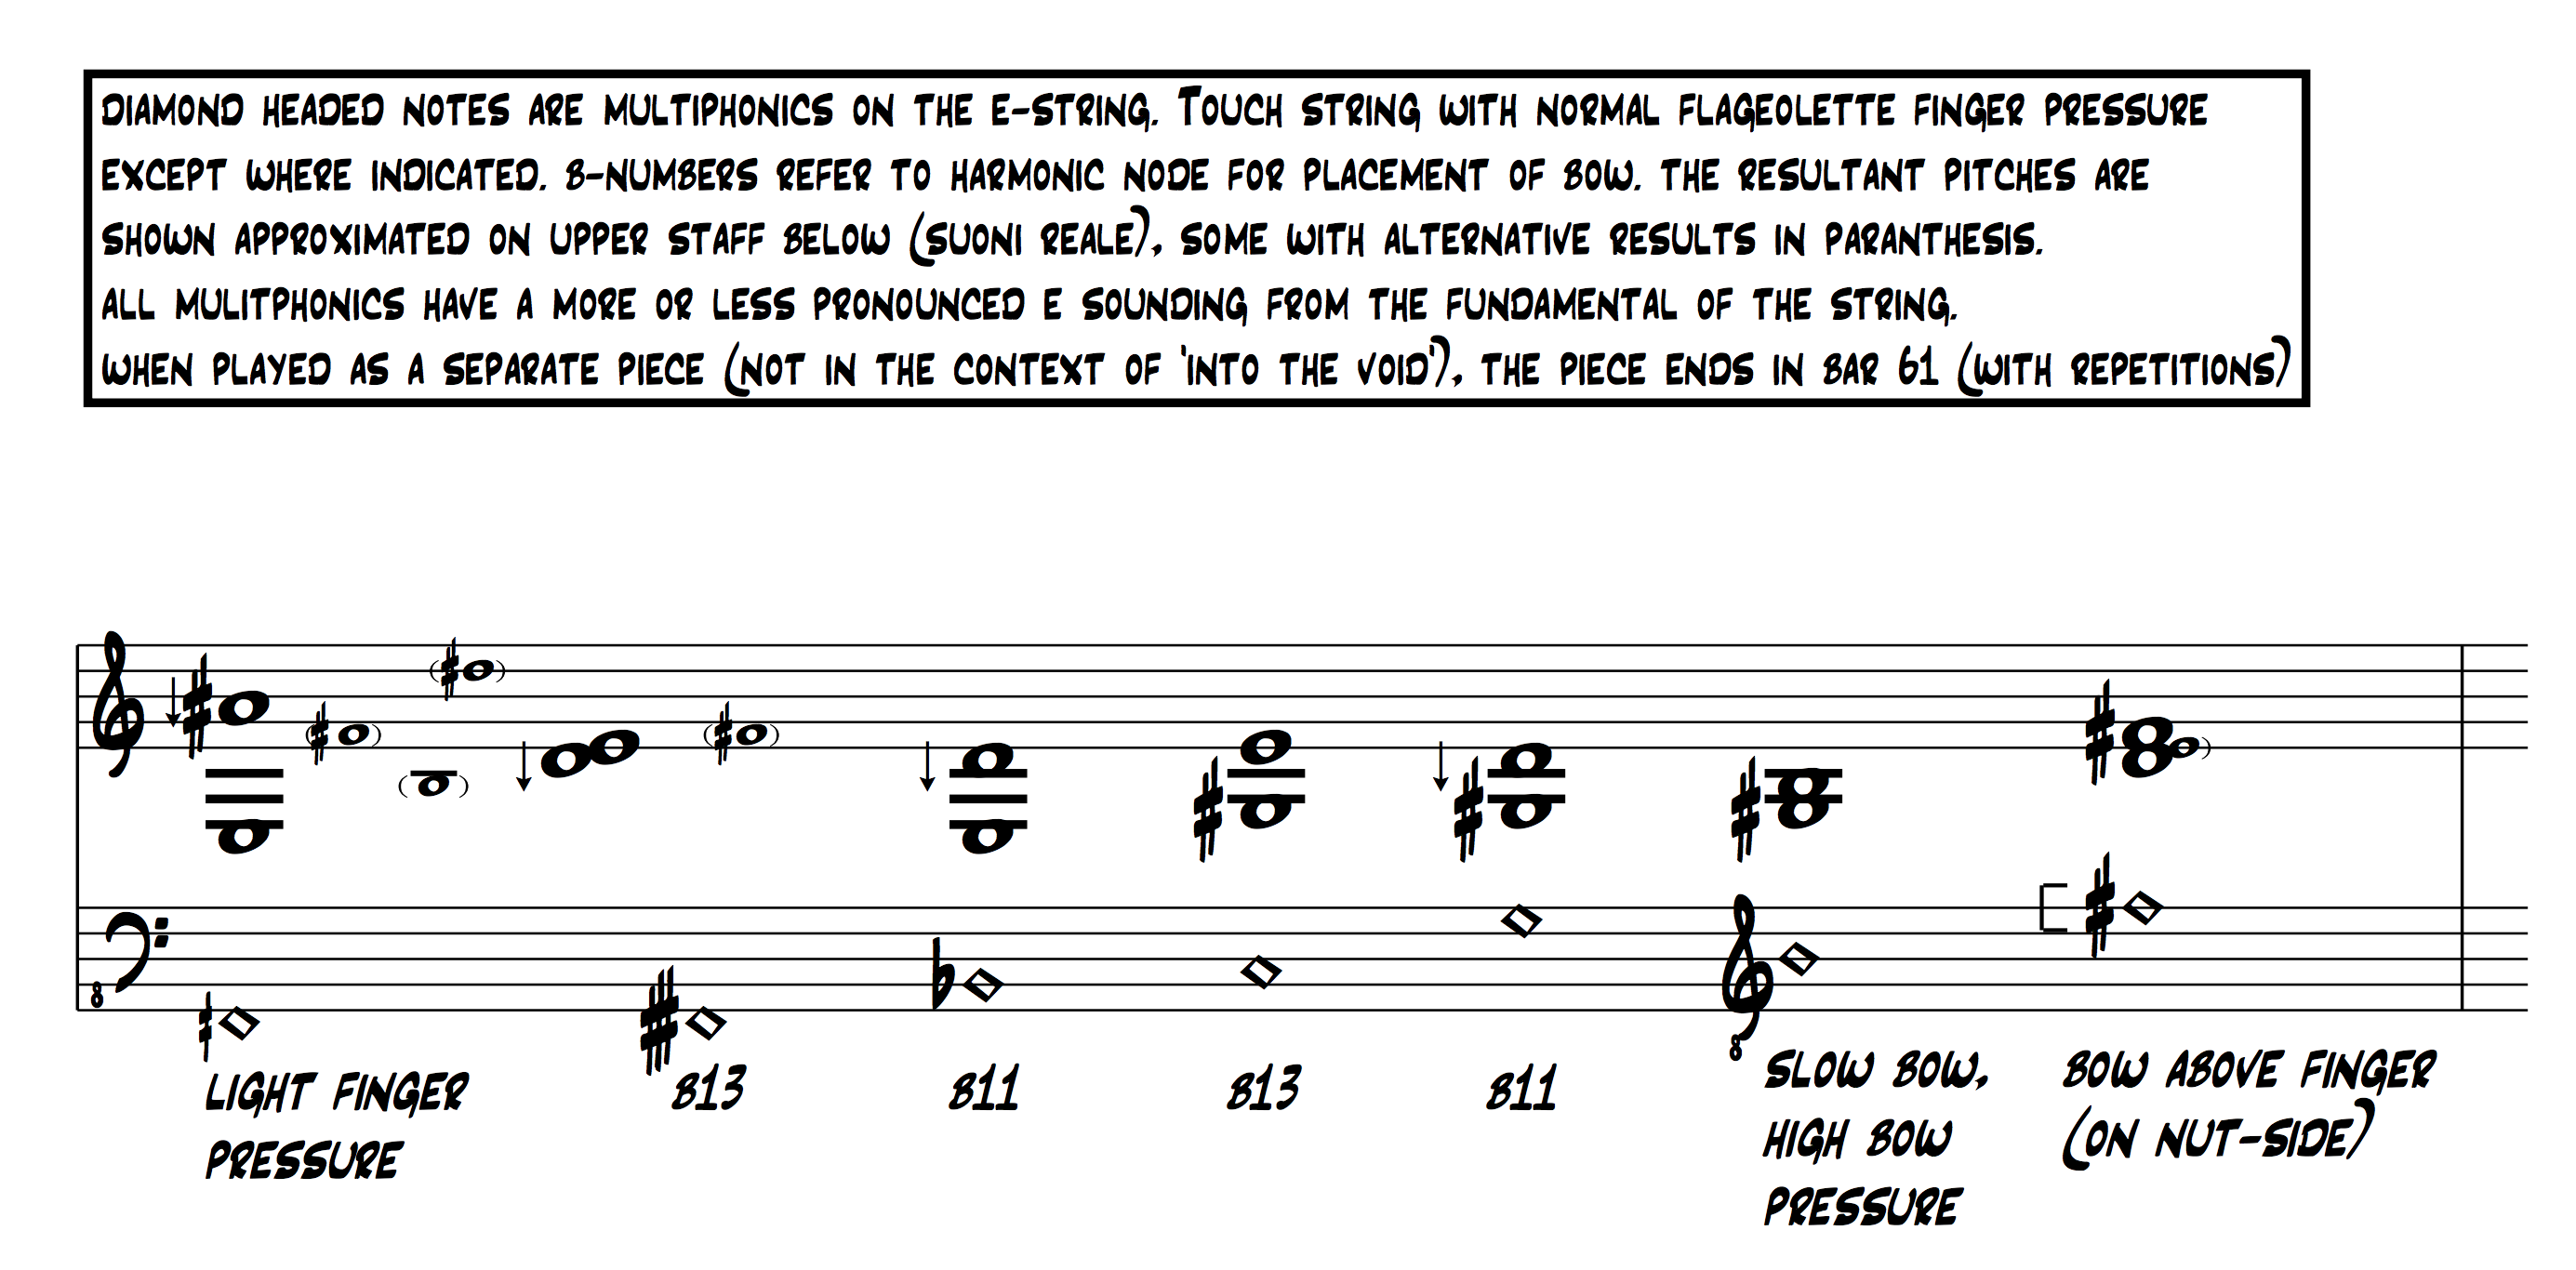
\includegraphics[width=\linewidth]{./resources/bueneMultiphonicNotation.png}
  \caption{Excerpt from Buene's Blacklight.}
\label{fig:Excerpt from Buene's Blacklight}
\end{figure}

Thelin's thesis on double bass multiphonics states:
\begin{quotation}
    `Multiphonics is [sic] always notated with the harmonic diamond sign, in tablature notation
indicating finger positions rather than musical pitches. I suggest using the symbol M. above or
below the note to indicate that it is a multiphonic sound, together with the indication on which
string to play the note (in Roman numerals).'\autocite[6]{thelinMultiphonicsDoubleBass2011}
\end{quotation}

\begin{figure}
    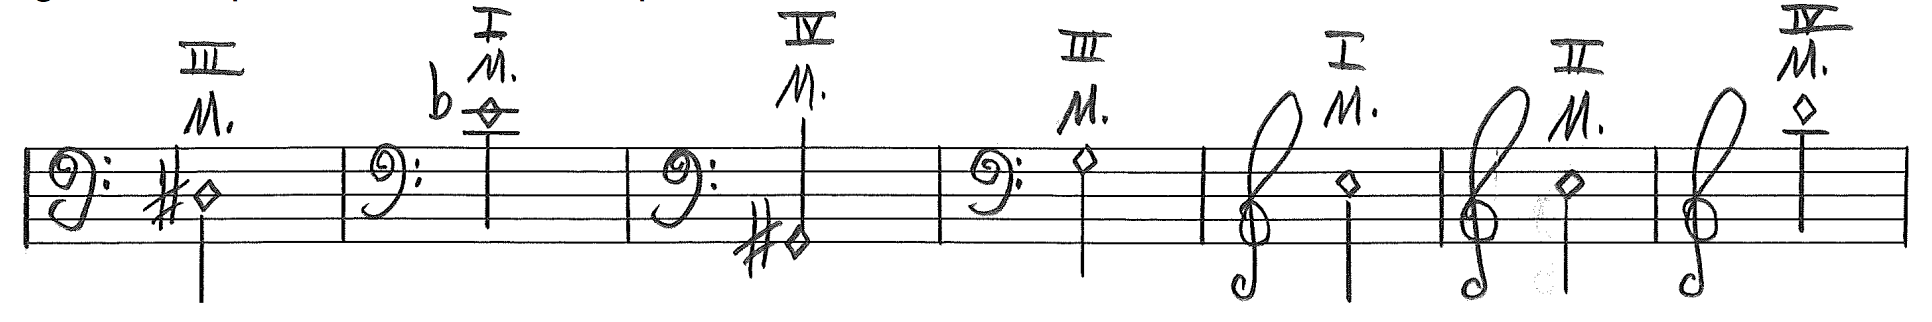
\includegraphics[width=\linewidth]{./resources/thelinMultiphonicNotation.png}
    % TODO: What is an excerpt from a thesis called? - https://trello.com/c/6xHaco1o/10-what-is-an-excerpt-from-a-thesis-called
    \caption{Excerpt from Thelin's thesis.}
  \label{fig:Excerpt from Thelin's thesis}
  \end{figure}
%   TODO: Reword Fallowfield dual harmonic positions
His notation suggestion is a somewhat less sophisticated version of Fallowfield's suggestion to notate the approximate pitch down to the cent necessary to produce the multiphonic. 
Due to the symmetry of the production of harmonics on the string, Fallowfield specifies both upper and lower positions necessary to produce the same multiphonic.\autocite[index/the-string/multiphonics-and-other-multiple-sounds/fingeringcharts.html]{fallowfieldCelloMap}
\begin{figure}
    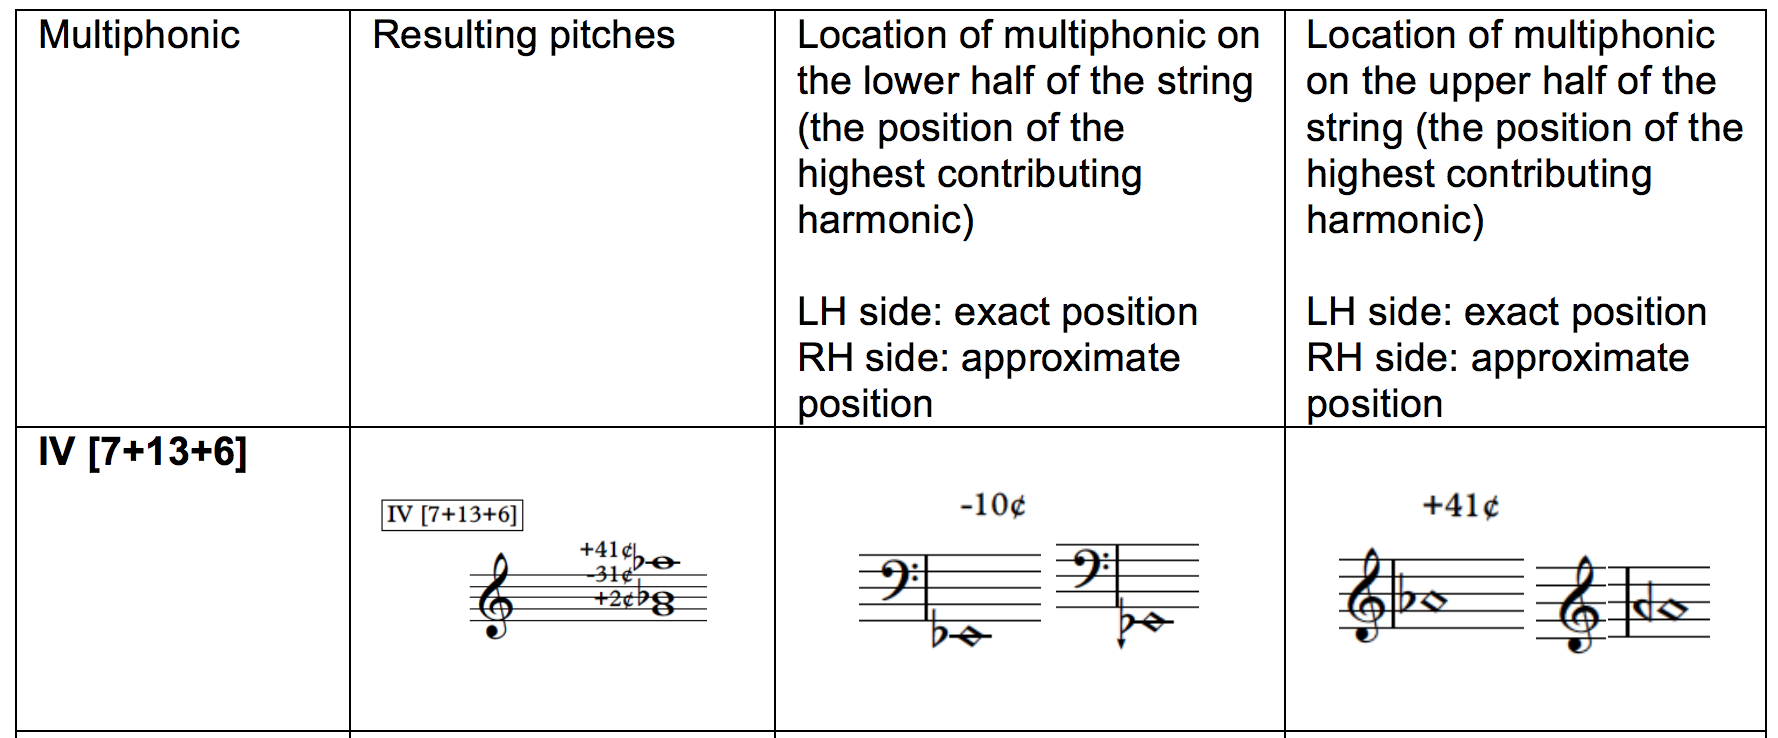
\includegraphics[width=\linewidth]{./resources/fallowfieldMultiphonicFingering.png}
    % TODO: What is an excerpt from a website called? - https://trello.com/c/04ESsMtJ/9-what-is-an-excerpt-from-a-website-called
    \caption{Excerpt from Fallowfields's website.}\autocite[]{fallowfieldCelloMap}
\label{fig:Excerpt from Fallowfields's website}
  \end{figure}

  We can see this in practice in Oliver Thurley's work for solo contrabass, \emph{yet another example of the porousness of certain borders}, where he adds another stave showing the intended pitches to be produced.\autocite{thurleyAnotherExamplePorousness2014}

  \begin{figure}
    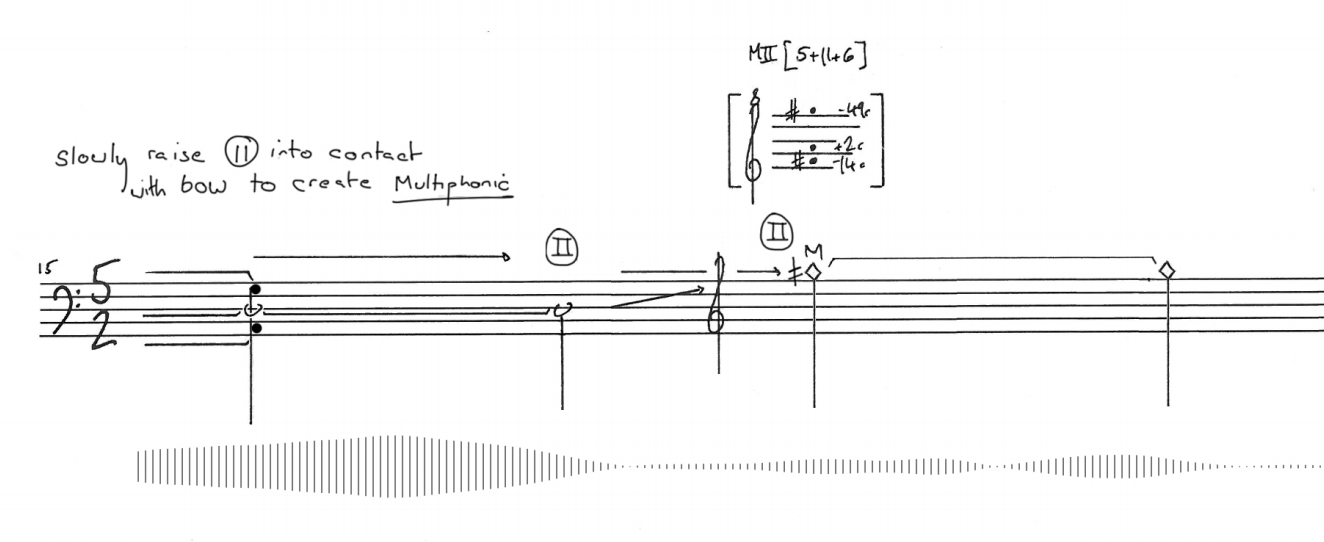
\includegraphics[width=\linewidth]{./resources/thurleyMultiphonicNotation.png}
    % TODO: What is an excerpt from a piece called? - https://trello.com/c/E9QqxFt0/12-what-is-an-excerpt-from-a-piece-called
    % TODO: Quotation marks in figure labels? - https://trello.com/c/HLJwnAwa/11-quotation-marks-in-figure-labels
    \caption{Excerpt from Thurley's \emph{yet another example of the porousness of certain borders}}
\label{fig:Excerpt from Thurley's `yet another example of the porousness of certain borders'}
  \end{figure}

Thurley embraces the fragility of these multiphonics, and uses their variability as a feature, rather than a hindrance. 
Slow, quiet transitions between multiphonics, double-stopped harmonics, and other extended techniques make the occasional unintentional destabilisation of a multiphonic a point of textural interest, rather than a flaw.

It becomes apparent through the examination of the literature surrounding multiphonics that they are still an emerging technique, but are not shrouded in mystery or disinformation as subharmonics are.

\newpage
\section{Half-Harmonics} \label{sec:halfHarmonicsDiscussion}
% TODO: Explain half-harmonics - https://trello.com/c/0v3lKvmZ/25-explain-half-harmonics
Half-harmonics is a term assigned to the fingering pressure found somewhere in between a regular note and harmonic. 
The technique is not difficult to produce, and the resultant sound is not dissimilar to the fragility of a multiphonic, producing both the fundamental pitch, and the harmonic. 
It should be noted that the half-harmonic is a modifying left-hand technique; it can be applied to multiphonics (although the resultant sound would likely be more noise than discernably either of the two techniques), but is not compatible with subharmonics due to the bow pressure needed to produce subharmonics eliminating the possibility of half-harmonics being produced.
The terminology has not been formalised, but is most widely known as half-harmonics, although some works describe the technique without ascribing a name.

Half-harmonics are explored in my work for violin, \nameref{sec:violinPiece}.

\subsection{Half-harmonics in the literature}
Half-harmonics, like the other techniques covered in this exegesis, have relatives in the wind and brass literature. 
Half-fingered and half-valved techniques appear in the respective nomenclature, and share common attributes of speaking poorly with bleedover into partials with the half-harmonic technique.
Unlike multiphonics, the mechanical production of the technique is not dissimilar to the wind and brass facsimiles; all three families' respective techniques revolve around pressing almost to the point of a \emph{normale} sound, but not quite, resulting in a pinched sound.
Because of this, it is not unreasonable to draw parallels between the half-valved and fingered literature, and half-harmonic literature. 

Half-harmonics do not feature heavily in the literature, with the most notable work being Sciarrino's 6 Caprices for solo violin.\autocite{sciarrinoCapricciViolino1976} 
It should be noted that Sciarrino wrote these in response to Paganini's caprices. 
They appear to take the same approach to composing in the same philosophy as New Complexicists, in the sense that the written score is the Platonic ideal, and that approximations are all that are expected.
This is supported by the fact that many performers play them as harmonics.

% TODO: add references for sciarrino claims - https://trello.com/c/7DtUyFWz/31-add-references-for-sciarrino-claims

Lachenmann also makes use of them, and states it is
\begin{quotation}
  [\dots] `important not to produce any harmonics here; the result should be a veiled, almost immaterial and hardly perceptible coloring of the dominating string sound produced by the stopped note'\autocite[foreword]{lachenmannMusikFurStreichquartett1972}
\end{quotation}
% Half-harmonics are used typically as a colourant, rather than a feature technique, and 

\begin{figure}
  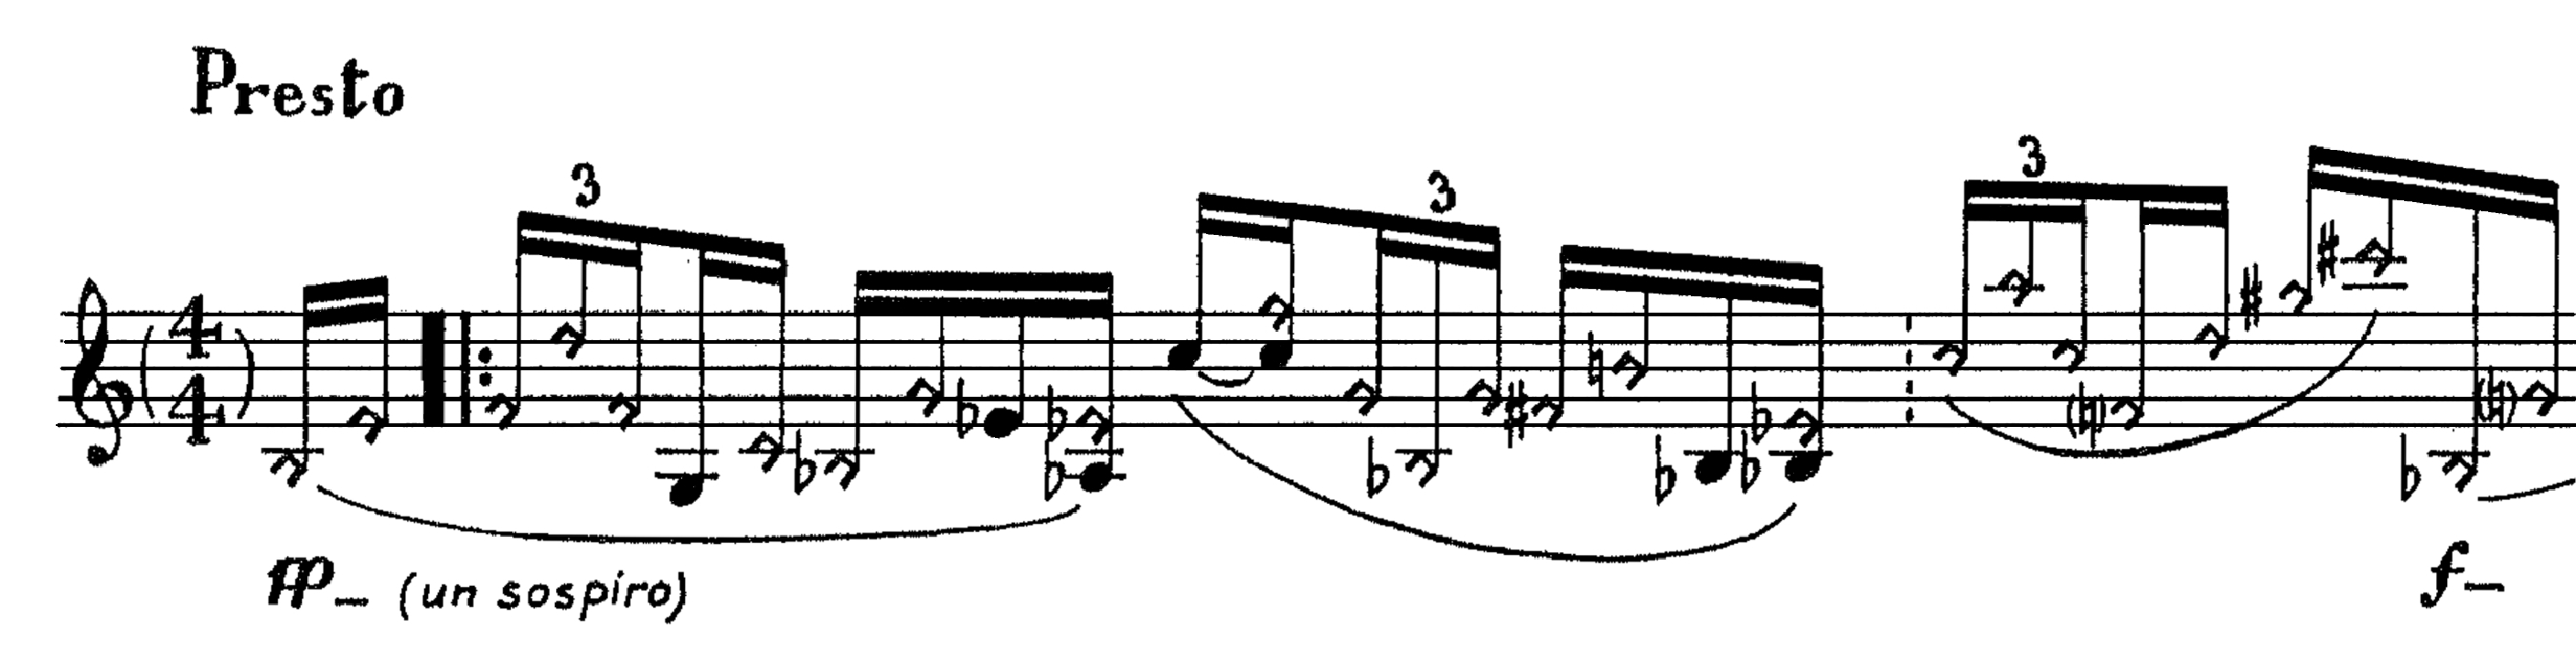
\includegraphics[width=\linewidth]{./resources/sciarrinoHalfHarmonicNotation.pdf}
  \caption{Excerpt from Sciarrino's 5th capriccio from \emph{6 Capricci for Violin}}
\label{fig:sciarrinoExcerpt}
\end{figure}

Sekulic adds to this quote, stating in \emph{Do you hear me?} that the stopped note:
\begin{quotation}
  `[\ldots] which, as indicated, is only lightly touched, in conjunction with the flautato bowing.'\autocite[28]{sekulicYouHearMe2012}
\end{quotation}

\subsection{Notation of half-harmonics in the literature}
Perhaps the most straight-forward technique covered in this exegesis, notation for half-harmonics have just a single variable of finger pressure to convey in notation.
The use of standard notation, modified to reflect the idea that the technique fits in 'half way between' two well established techniques (normale and harmonics) would be ideal, conforming to Gould's ideology of maintaining uniformity.



% TODO: Add Gould reference for creating new notation - https://trello.com/c/pAR2S6wg/26-add-gould-reference-for-creating-new-notation
% chapter3.tex (Chapter 3 of the thesis)


\chapter{Compositions and Implementation of Techniques}
This is where I will present my findings and draw conclusions on the various techniques that I explored through writing and workshopping in Chapter 2. This will be more broad, and I will make amendments to what I posited in Chapter 2. \lipsum[5]
\subsection{Background}
Provide a better understanding on the ways that these techniques can be incorporated idiomatically into a composer's practice.

\subsection{Research statement/problem}
There is a dearth of resources for composers interested in these techniques, as evidenced by this research being novel.

\subsection{Aim and scope of thesis}
Ways to incorporate and present these techniques in an idiomatic way that is intuitive.

\subsection{Significance of work}
The properties of these techniques and the ways that they can be used idiomatically.


\lipsum[4]

My folio of works comprises of four pieces. `Doppelganger', for solo viola, `The Veldt', for solo contrabass, `Placeholder', for solo cello, and `what are you doing with the humans', for violin. 
These works all deal with different facets of the techniques that I have researched in this exegesis. 
Through the process of practice based research and reflection on the implementation of these pieces, it is hoped that a clear identity of idiomatic treatment of these techniques will be elucidated.
Shortcomings are still valuable data points due to the lack of information readily available about the treatment and usage of these techniques.
It is envisaged that these works are to be used as etudes, both for musicians as testing grounds for the capabilities of the techniques, and for composers seeking to study scores to better understand how to implement these techniques in their own works.
Through the process of journalling my compositional intent, it will become clear what the function of each piece is.
Comparisons and contrasts to pre-existing literature and works will support the techniques' idiomacy. 


\subsection{Background}
Implement the experiments in a musical context.
\subsection{Research statement/problem}
Compositions will show both how these techniques can be used idiomatically, and how they can inform my craft.
\subsection{Aim and scope of thesis}
Writing works which will increase the collective understanding of how to implement these techniques.
\subsection{Significance of work}
Incorporating these techniques into my compositional process will show the pitfalls and ways that these techniques can be used.

\section{`what are you doing with the humans'}
\emph{what are you doing with the humans} is a solo work for violin that explores half-harmonics.
It is a non-programmatic work, and the title was inspired by a question that my supervisor posed to me while I sought ethics approval for the exegesis.
Half-harmonics are perhaps one of the simplest techniques to achieve, produced by applying finger pressure halfway between that required to create a harmonic, and a \emph{normale} sound.
This means that the scale of finger pressure is thus;

\begin{table}[]
    \centering
    \caption{Finger Pressure \& Resultant Sound}
    \label{tab:finger-pressure}
    % \resizebox{\textwidth}{!}{%
    \begin{tabular}{@{}ll@{}}
    \toprule
    Finger pressure & Result        \\ \midrule
    Open            & Fundamental   \\
    Touching        & Harmonic      \\
    More pressure   & Half-harmonic \\
    Fingerboard     & Normale       \\ \bottomrule
    \end{tabular}%
    % }
    \end{table}

The one-dimensional nature of this facet of the techniques leaves little variability in the implementation of the technique. 
Thus, \emph{what are you doing with the humans} explores the relationship between half-harmonics and other finger pressures. 
Rapid change between half-harmonics, regular harmonics, and \emph{normale} makes the work an exercise in finger control, as well as an introductory work to half-harmonics.
Below, I demonstrate the rapid changes of the half-harmonics.

% TODO: Add in picture of half harmonics  - https://trello.com/c/cYTkFAaV/27-add-in-picture-of-half-harmonics
Picture goes here

\emph{what are you doing with the humans} takes inspiration from Sciarrino's fifth Caprice, and serves as a stepping stone to the more difficult Caprice.\autocite[]{sciarrinoCapricciViolino1976} 
In practice, the pitch content of my work was obscured by the glassy texture of half-harmonics, rendering large portions of it as noise. 
With the knowledge that properly performed, the harmonic content would be obscured, I leant into this, writing in a more tonal style than I do usually.


Another facet of half-harmonics that I wanted to explore was the timbral aspect of them, bar 67 shown below.
Similar to a multiphonic in their rich harmonic content, half-harmonics do not have the purity of tone that regular harmonics have.
I explore the interplay of half-harmonics, regular harmonics, and \emph{normale}, double stopped minims and semibreves slowly changing from one mode of pressure to another.
In this way, violinists that play \emph{what are you doing with the humans} will become familiar with different modes of pressure played concurrently.

\section{`Doppelganger'}
% TODO: Write Doppelganger
\emph{Doppelganger} is a piece for solo viola, written to explore the lower register of the viola using subharmonics juxtaposed with upper harmonics. 


\subsection{Findings of \emph{Doppelganger}}
Workshopping an early draft of \emph{Doppelganger} with a violist, I found that the pressure needed to `find' a  \lipsum[3]

\section{`The Veldt'}
% TODO: Write The Veldt
Inspired by the eponymous short story by Ray Bradbury, \textit{The Veldt} is a composition for solo contrabass with electronics. 
Similarly like the namesake, this world is filled with danger but also beauty. 
It is non-programmatic, and my intent with Veldt was to create a soundworld and space that the performer was able to `roam around' in, and features several sections of improvisation on pitch-sets.

\subsection{Findings of \emph{The Veldt}}
Writing for contrabass, I found 

% chapter4.tex (Chapter 4 of the thesis)

\chapter{Findings}
This is where I will be presenting my research as a manual for composers. 
It will follow the Dick model of categorization.\autocite{dickOtherFlute1989} 
It will also take into account how common the technique is, as well as notational challenges.

\subsection{Subharmonics}
Subharmonics are a difficult technique, that lend themselves to solo works, or works where they can be brought to the forefront.
They are notably different to overpressure, but bleed over into non-pitched overpressure is common.

This, plus the difficulty in their execution, makes them unsuitable for melodic content.

Players may find that subharmonics are easier on older strings, and they may also find that adding twists to the string may also help, or hinder the production of subharmonics, referencing the table below. Composers seeking to make use of subharmonics extensively may wish to consider the below table.

\begin{table}[]
    \centering
    \resizebox{\textwidth}{!}{%
    \begin{tabular}{llllllll}
    \hline
    \multicolumn{1}{r}{\begin{tabular}[c]{@{}r@{}}number of twists/\\ subharmonic intervals\end{tabular}} & \multicolumn{1}{c}{1/2} & \multicolumn{1}{c}{1} & \multicolumn{1}{c}{2} & \multicolumn{1}{c}{3} & \multicolumn{1}{c}{4} & \multicolumn{1}{c}{5} & \multicolumn{1}{c}{6} \\ \hline
    minor 2nd                                                                                             & x                       & x                     &                       &                       &                       &                       &                       \\
    major 2nd                                                                                             & x                       & x                     &                       &                       &                       &                       &                       \\
    minor 3rd                                                                                             & x                       & x                     & x                     &                       &                       &                       &                       \\
    major 3rd                                                                                             & x                       & x                     & x                     & x                     &                       &                       &                       \\
    perfect 4th                                                                                           &                         &                       &                       & x                     & x                     &                       &                       \\
    dim. 5th                                                                                              &                         &                       &                       &                       & x                     & x                     &                       \\
    perfect 5th                                                                                           & x                       &                       &                       &                       &                       & x                     & x                     \\
    minor 6th                                                                                             &                         &                       &                       &                       &                       &                       & x                     \\
    octave                                                                                                & x                       & x                     & x                     & x                     & x                     &                       &                      
    \end{tabular}%
    }
    \end{table}

Composers looking to use this technique should be aware that it is not a standard technique, and instrumentalists will need copious amounts of practice and guidance in order to fully realise this technique.

\subsubsection{Notation of Subharmonics}
Subharmonics should be notated with a square notehead, and a small notehead (optionally in parenthesis) at the desired pitch.
The technique description and notation should be included in the performance notes.

\subsection{Multiphonics}
Multiphonics are easier to achieve on larger instruments, due to the need for precise ratio-based fingering to achieve the resonance of multiple partials.
The technique description and notation should be included in the performance notes.
\lipsum[4]

\subsubsection{Notation of Multiphonics}

\subsection{Half-harmonics}

\subsubsection{Notation of Half-harmonics}
Half-harmonics 
The technique description and notation should be included in the performance notes.

\section{Reflection}




\lipsum[4]
% Conclusion
% These techniques are underrepresented because of a variety of reasons, one of them being that there is a lack of resources dedicated to writing for them.
% It is hoped that this exegesis will contribute to their more widespread adoption. 
% It becomes apparent that the literature surrounding these techniques still lacks comprehensive guidelines over the techniques' use, and the works that have been produced have been through trial and error.
\section{Impact and Further Research}
This exegesis will help inform other artists interested in implementing these techniques. 
Compositionally, the scope of this exegesis has been limited to the techniques in a soloistic context, and no research into how the techniques fit into an ensemble context has been done as of the time of writing.
The exact mechanics of the production of \hyperref[sec:subharmonics]{subharmonics} and \hyperref[sec:multiphonics]{multiphonics} are still poorly understood.
Further research into the way the techniques react to artificial harmonics, the difference between the two nodal points for multiphonics, and the methods for producing different intervals of subharmonics is needed for a holistic understanding.
The analysis and cataloguing of the qualities of each multiphonic and subharmonic would contribute further to the ideal of idiomatic writing for the techniques.


\addcontentsline{toc}{chapter}{Conclusion}
\section{Conclusion}
It becomes apparent that the literature surrounding these techniques is still in its infancy, with few sources of authority due to the niche nature of the techniques.
In this exegesis, the documentation of the existing literature and findings from the implementation of the techniques has helped establish a baseline of how to treat these techniques, which others can build upon.
Through the gradual adoption of these techniques, a standardised notation will form, and further proliferate the acceptance of these techniques in modern literature.



\backmatter{}
\begin{appendixes}
    \include{backmatter/appendixa}
    \include{backmatter/appendixb}
\end{appendixes}

\printbibliography{}

\end{document}
